% Copyright (c) 2026 Islam Ibrahim. All rights reserved.

\documentclass[tikz,border=10pt]{standalone}
\usepackage[T1]{fontenc}
\usepackage{lmodern}
\usepackage{amsmath}
\usepackage{tikz}
\usetikzlibrary{arrows.meta,decorations.pathmorphing}

\begin{document}
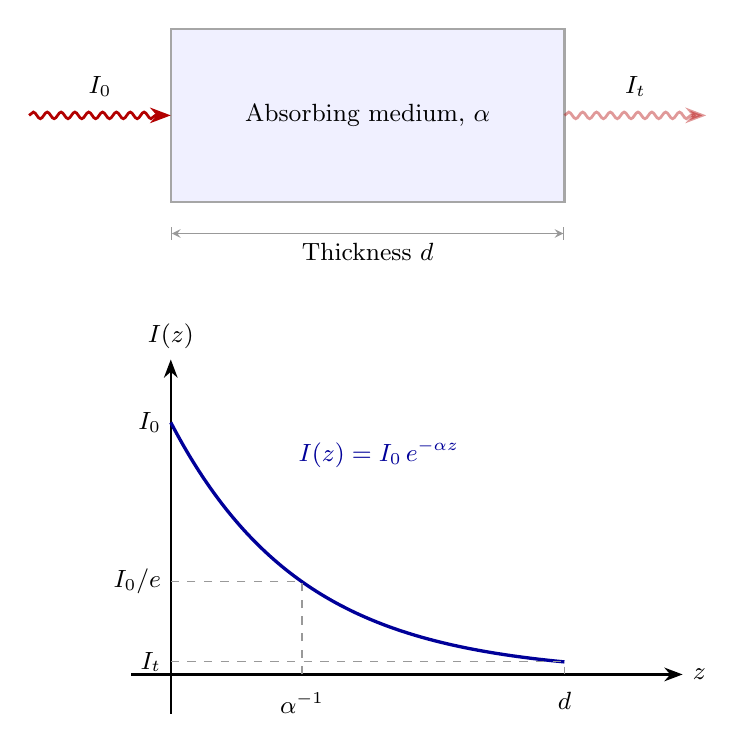
\begin{tikzpicture}[font=\small\rmfamily, >=Stealth]

  \def\d{5}
  \def\H{2.2}
  \def\Izero{3.2}
  % Renamed to \myalpha so we don't overwrite the LaTeX Greek letter macro
  \def\myalpha{0.6} 
  
  \pgfmathsetmacro\Id{\Izero*exp(-\myalpha*\d)}
  \pgfmathsetmacro\zdelta{1/\myalpha}
  \pgfmathsetmacro\Ie{\Izero*exp(-1)}

  \begin{scope}[shift={(0, 4.5)}]
    \fill[blue!6, draw=gray!70, line width=0.8pt] (0, 0) rectangle (\d, \H);
    \node at (\d/2, \H/2) {Absorbing medium, $\alpha$};

    \draw[|<->|, >=stealth, gray!80] (0, -0.4) -- (\d, -0.4) node[midway, below, text=black] {Thickness $d$};

    \draw[->, line width=1pt, red!70!black, decorate, decoration={snake, amplitude=1.2pt, segment length=5pt, post length=4pt}] (-1.8, \H/2) -- (0, \H/2) node[midway, above=3pt, text=black] {$I_0$};
    \draw[->, line width=1pt, red!70!black, opacity=0.4, decorate, decoration={snake, amplitude=1.2pt, segment length=5pt, post length=4pt}] (\d, \H/2) -- (\d+1.8, \H/2) node[midway, above=3pt, text=black, opacity=1] {$I_t$};
  \end{scope}

  \begin{scope}[shift={(0, -1.5)}]
    \draw[->, line width=0.8pt] (-0.5, 0) -- (\d + 1.5, 0) node[right] {$z$};
    \draw[->, line width=0.8pt] (0, -0.5) -- (0, \Izero + 0.8) node[above] {$I(z)$};

    \draw[line width=1.2pt, blue!60!black, domain=0:\d, samples=100] plot (\x, {\Izero*exp(-\myalpha*\x)});

    \node[left] at (0, \Izero) {$I_0$};
    
    \draw[dashed, gray!80] (0, \Id) node[left, text=black] {$I_t$} -- (\d, \Id) -- (\d, 0) node[below=3pt, text=black] {$d$};
    \draw[dashed, gray!80] (\zdelta, 0) node[below=3pt, text=black] {$\alpha^{-1}$} -- (\zdelta, \Ie) -- (0, \Ie) node[left, text=black] {$I_0/e$};
    
    \node[right, blue!60!black] at (1.5, \Izero - 0.4) {$I(z) = I_0 \, e^{-\alpha z}$};
  \end{scope}

\end{tikzpicture}
\end{document}